\documentclass[a4paper]{letter}
\usepackage{wallpaper}
\usepackage{geometry}
\usepackage{xcolor}
\usepackage[T1]{fontenc}
\usepackage[scaled]{helvet}
\usepackage{fontawesome5}
\usepackage[hidelinks]{hyperref}
\usepackage[french]{babel}
\usepackage{graphicx}
\usepackage{tikz}
\usepackage{setspace}
\usepackage{comment}
\usepackage{eso-pic}


\usetikzlibrary{calc}

\renewcommand{\familydefault}{\sfdefault}

\geometry{
  a4paper,
  left=20pt,
  right=20pt,
  top=0pt,
  bottom=0pt,
  nohead,
  nofoot,
  nomarginpar
}




% Custom command for dividers
\newcommand{\divider}{\rule{\linewidth}{0.9pt}}

% ============================================================
% ======================== Left Side =========================
% ============================================================


\begin{document}
\AddToShipoutPictureBG*{
  \AtPageLowerLeft{
    % Adjust the horizontal shift with \hspace:
    \hspace*{-5mm}% Move 1 cm to the left
    
\includegraphics[width=\paperwidth]{cvbg.png}%
  }
}

%\small
\begin{minipage}[t]{0.30\textwidth}
\setstretch{1.2} 
\setlength{\baselineskip}{1\baselineskip}
\color{white}
\vspace{5mm}


% ========================== Photo ============================

\begin{tikzpicture}
    \clip (0,0) circle (2cm);
    \node[anchor=center] at (0,0) {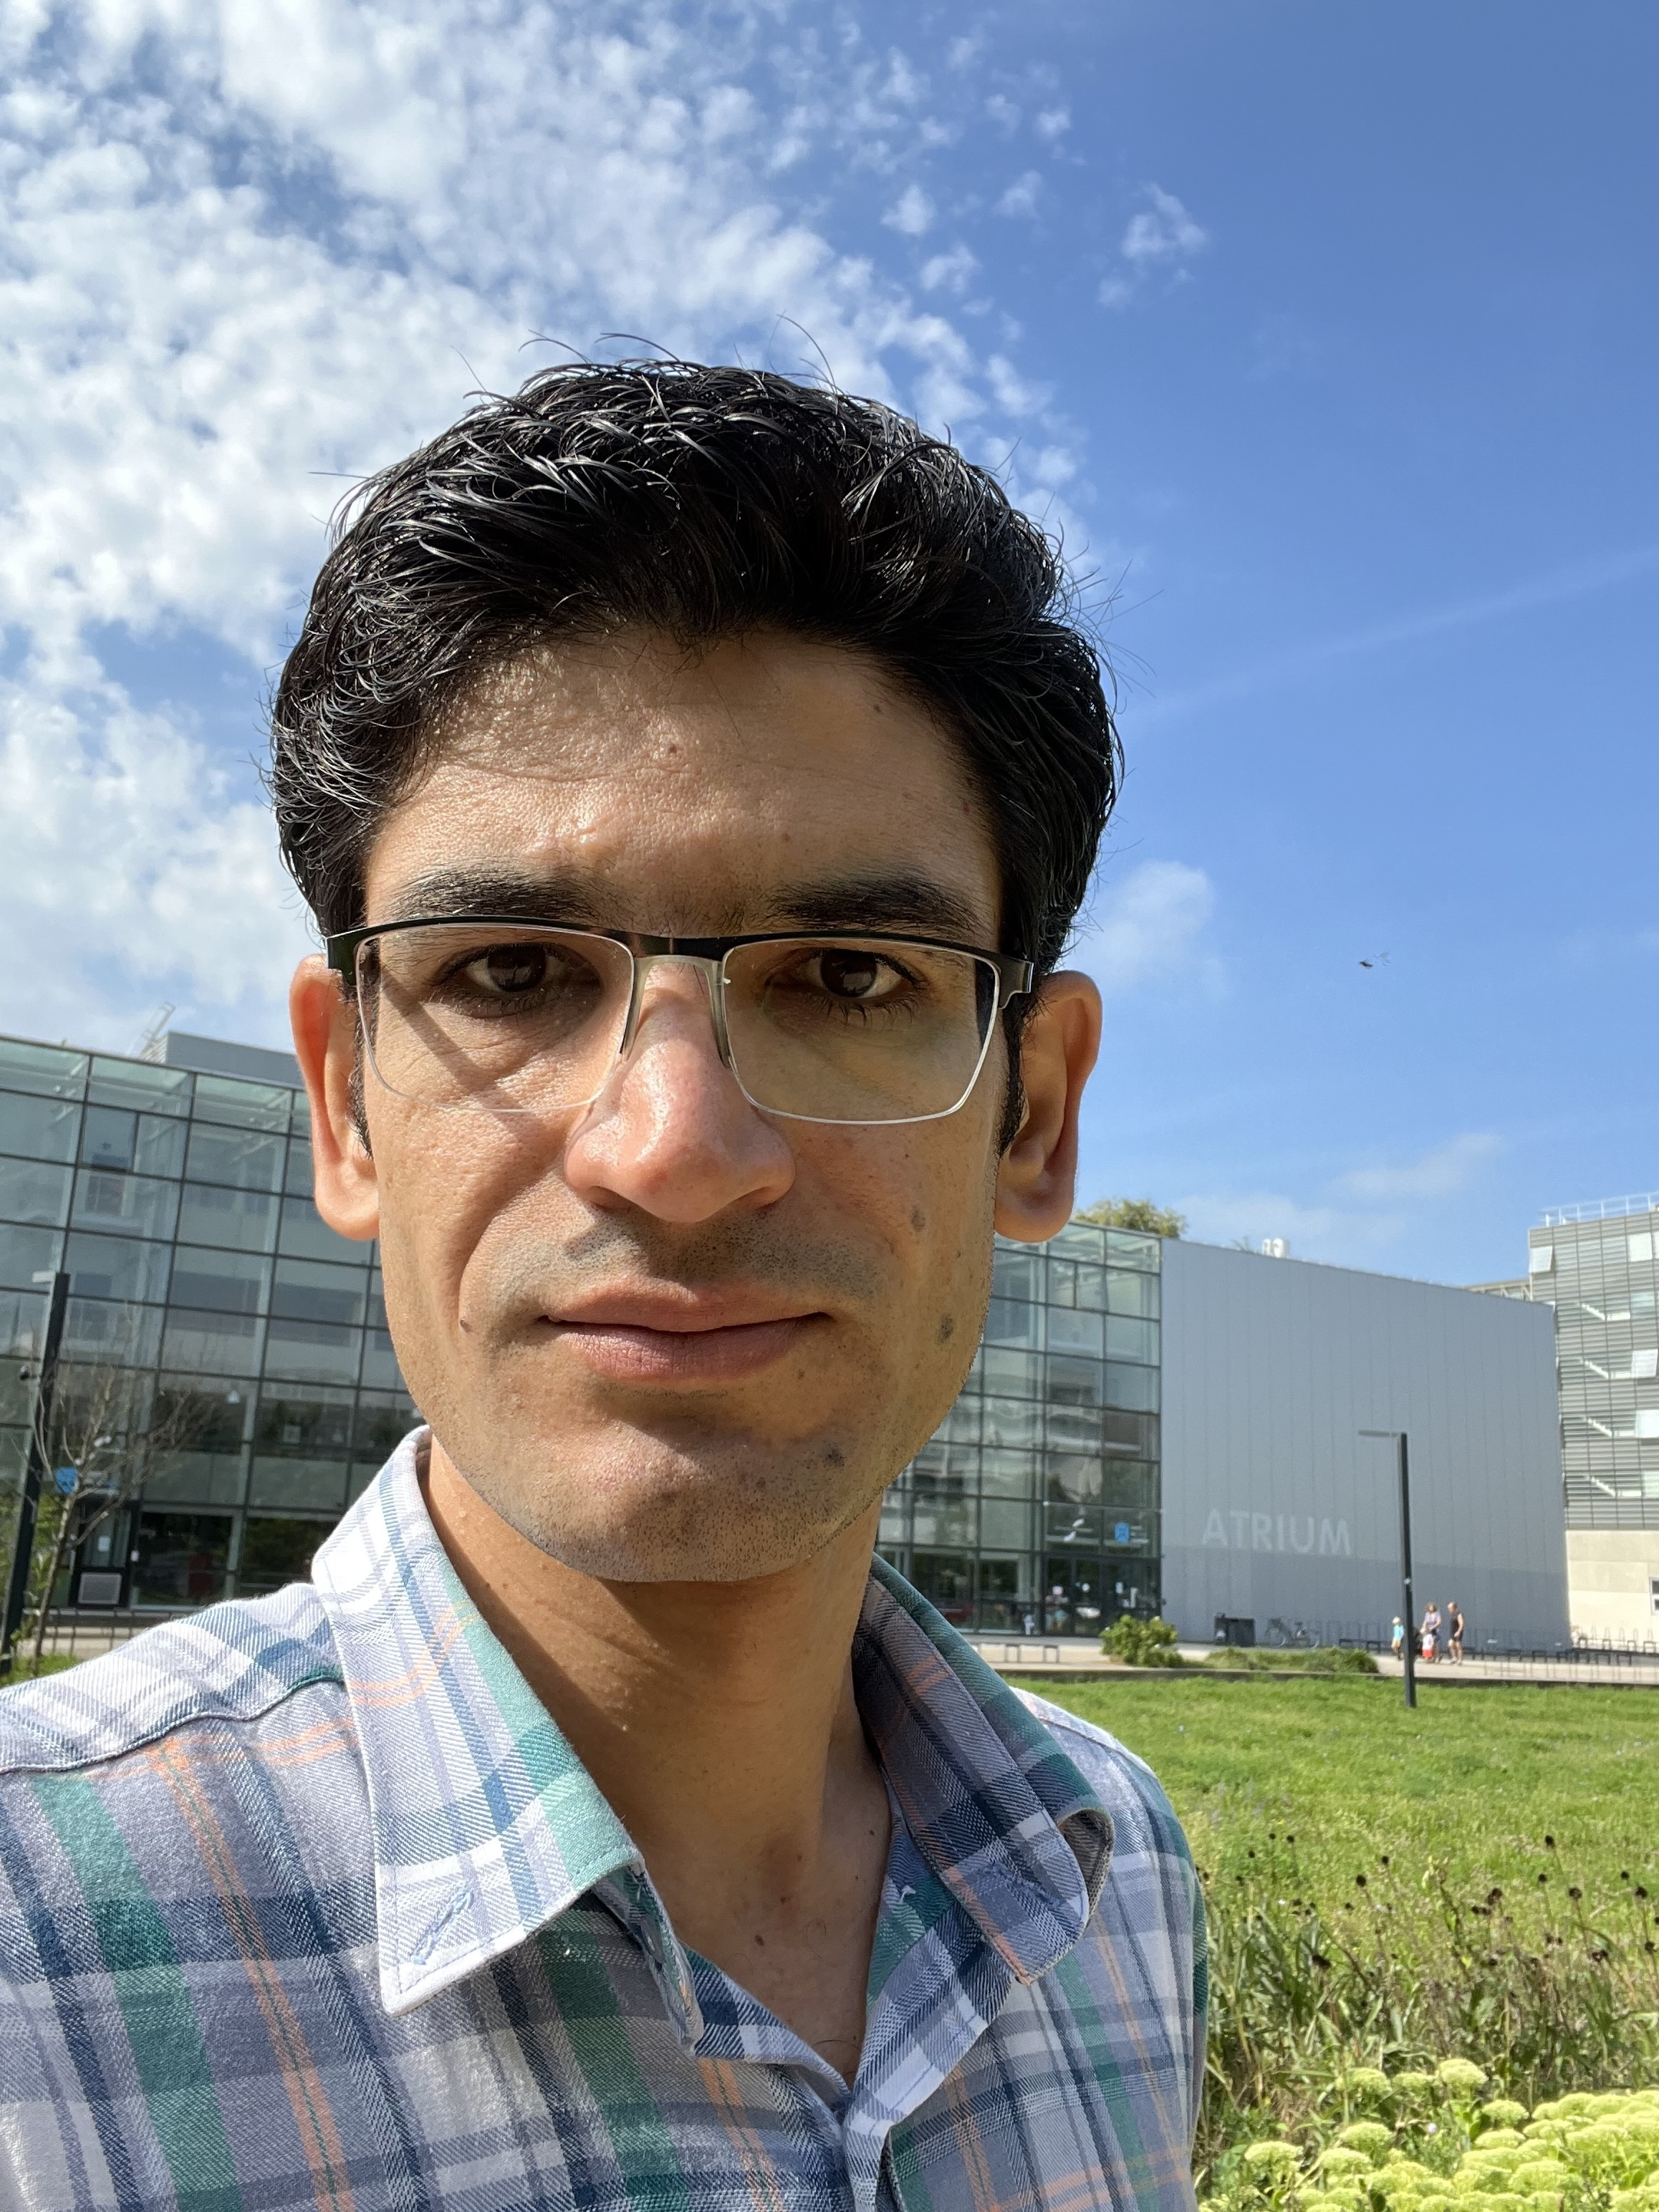
\includegraphics[width=4cm]{profile.jpg}};
\end{tikzpicture}

\vspace{5mm}

\divider

% ========================= Contact ===========================

\faPhone \quad 06 52 22 49 24

\faEnvelope \quad jafarizadeh89@gmail.com

\faGithub \quad \href{https://github.com/jafarizadeh}{jafarizadeh}

\faLinkedin \quad \href{https://www.linkedin.com/in/jafarizadeh/}{linkedin.com/in/jafarizadeh/}


\divider

% ================ Languages ================
{\large \textbf{Languages}}

\faCircleNotch \quad Persian (native language)

\faCircleNotch \quad French (advanced level)

\faCircleNotch \quad English (intermediate level)

\divider

% ================ Programming Languages ================

{\large \textbf{Programming Languages}}

\faCircleNotch \quad Python

\faCircleNotch \quad C

\faCircleNotch \quad Swift

\faCircleNotch \quad HTML / CSS

\faCircleNotch \quad JavaScript

\faCircleNotch \quad SQL

\divider

% ===================== CAD Software ======================

{\large \textbf{CAD Software}}

\faCircleNotch \quad AutoCAD

\faCircleNotch \quad CATIA

\divider

% ========================== Networking ==========================

{\large \textbf{Networking}}

\faNetworkWired \quad CCNP Security (in progress)

\faNetworkWired \quad CCNP-ENCOR

\faNetworkWired \quad CCNP-ENARSI

\faNetworkWired \quad CCNA

\divider

% ===================== Driving License ======================

{\large \textbf{Driving License}}

\faCar \quad B2 License

\divider

% ===================== Interests ======================

{\large \textbf{Interests}}

\faBicycle \quad Cycling

\faGamepad \quad Video games (Minecraft)



\end{minipage}
\hspace{2mm}
\begin{minipage}[t]{0.67\textwidth}




% ============================================================
% ======================= Right  Side ========================
% ============================================================

\setlength{\baselineskip}{1.4\baselineskip}
\vspace{0.7cm}

{\huge Mehdi JAFARIZADEH}

\vspace{0.5cm}
% ========================= Education =========================

{\large \textbf{Education}}
\divider

{\textbf{Bachelor's Degree (3rd Year) in Computer Science}}

{\footnotesize September 2021 - Present}

{\textit{University of Strasbourg, Strasbourg}}

\vspace{1mm}

\begin{itemize}
    \footnotesize
    \item Skills acquired: configuration and management of LAN/WAN networks,
    process management, Linux administration, complexity analysis, data structures.
\end{itemize}

\vspace{2mm}

{\textbf{Bachelor's in Energy Engineering (Equivalent to Bachelor's Degree)}}

{\footnotesize September 2014 - December 2018}

{\textit{Quchan University of Technology, Mashhad, Iran}}

\vspace{1mm}

\begin{itemize}
    \footnotesize
    \item Final Year Project: Energy Consumption in Smart Homes
    \item Skills acquired: Energy modeling, Energy efficiency optimization, Use of specialized software
\end{itemize}

\vspace{2mm}

{\textbf{Diploma in Accounting (2-Year Degree)}}

{\footnotesize September 2007 - December 2010}

{\textit{Azad University of Kerman, Kerman, Iran}}

\vspace{1mm}
\begin{itemize}
    \footnotesize
    \item Skills acquired: Financial analysis, Regulatory compliance
\end{itemize}
\vspace{3mm}

% ================ Additional Training ==================

{\large \textbf{Additional Training}}
\divider
\vspace{4mm}
\begin{itemize}
    \footnotesize \item {\textbf{CCNP ENCOR 350-401:} Infrastructure architecture, security, and automation; (173 h)}
    \vspace{2mm}
    \footnotesize \item {\textbf{CCNP ENARSI 300-410:} Advanced routing EIGRP, OSPF, BGP, and WAN networks; (134 h)}
    \vspace{2mm}
    \footnotesize \item {\textbf{CCNA 200-301:} Network fundamentals, configuration, and troubleshooting; (128 h)}
\end{itemize}
\vspace{3mm}


% ================ Professional Experience =================

{\large \textbf{Professional Experience}}
\divider

\vspace{1mm}
{\textbf{Internship: IT Department}}

{\footnotesize May 2010 - September 2010}
\begin{itemize}
    \footnotesize \item \textit{Aria-Etemad Accounting Firm}
   \newline
    Performed client accounting calculations using Microsoft Office, particularly Excel. Developed advanced skills in Microsoft 365.
\end{itemize}

\vspace{3mm}
{\textbf{Internship: Research and Development Department}}

{\footnotesize June 2017 - September 2017}
\begin{itemize}
    \footnotesize \item \textit{Kerman and Kavian Cable Industry}
   \newline
   Conducted research on thermal analysis and electrical conductivity of copper wires under the supervision of Dr. Abdollahi, using ANSYS and SolidWorks for modeling and analysis of technical data, accompanied by an in-depth study of scientific articles.
\end{itemize}

\vspace{3mm}
{\textbf{Network Security Technical Assistant}}

{\footnotesize November 2023}
\begin{itemize}
   \footnotesize \item \textit{GOHARYAN SASU, Strasbourg}
   \newline
   Assisted the technical team in setting up and configuring secure communication channels (VPN and IPSec) as part of an international collaboration. Contributed significantly to protecting sensitive research communications.
\end{itemize}

\vspace{3mm}
{\textbf{Director of the Energy Engineering Association}}

{\footnotesize September 2015 - December 2017}
\begin{itemize}
   \footnotesize \item \textit{Quchan University of Technology, Mashhad}
   \newline
   Conducted educational courses and organized scientific competitions within the Energy Engineering Association to promote renewable energy and raise awareness of energy efficiency challenges.
\end{itemize}

\vspace{3mm}

{\textbf{Teaching Assistant}}

{\footnotesize September 2014 - December 2017}
\begin{itemize}
    \footnotesize \item \textit{Quchan University of Technology, Mashhad}
    \newline
    Teaching assistant for Mathematics 1, Mathematics 2, and Energy Conversion: supported students, explained key concepts, and assisted in preparing tutorials and exams.
\end{itemize}

\vspace{3mm}


{\large \textbf{Academic Contributions}}
\divider
\vspace{3mm}
\begin{itemize}
    \footnotesize \item {\textbf{Co-author}, \textit{Energy Audit Guide for Quchan University of Technology students, with Dr. Majid Mahdavian, Published in 2019}}



\end{itemize}



\end{minipage}

% ========================== Code QR ==========================

\begin{tikzpicture}[remember picture,overlay]
    \node[anchor=south east,inner sep=0pt] at ($(current page.south west)+(6.1cm,+2.5cm)$) {
        
\includegraphics[width=2cm]{Documentation_FR.png}
    };
    
    \node[anchor=south east,inner sep=0pt] at ($(current page.south west)+(3.8cm,+2.5cm)$) {
        \begin{minipage}[t]{3.05cm} 
            \color{white} \scriptsize \href{https://drive.google.com/file/d/1jKjZWYadaikaPetkEmjoupWWh_w1sMKA/view?usp=drive_link}{Please click here or scan this QR code to access a detailed folder of my academic and professional contributions.}
        \end{minipage}
    };


    \node[anchor=south west,inner sep=0pt] at ($(current page.south west)+(0.8cm,1cm)$) {
        \begin{minipage}[t]{4cm}
            \tiny \textcolor{white}{Dernière mise à jour: \today}
        \end{minipage}
    };
\end{tikzpicture}

\end{document}
